%% \begin{figure*}[!h]
%%   \centering
%%   \begin{subfigure}[t]{0.3\textwidth}
%% 	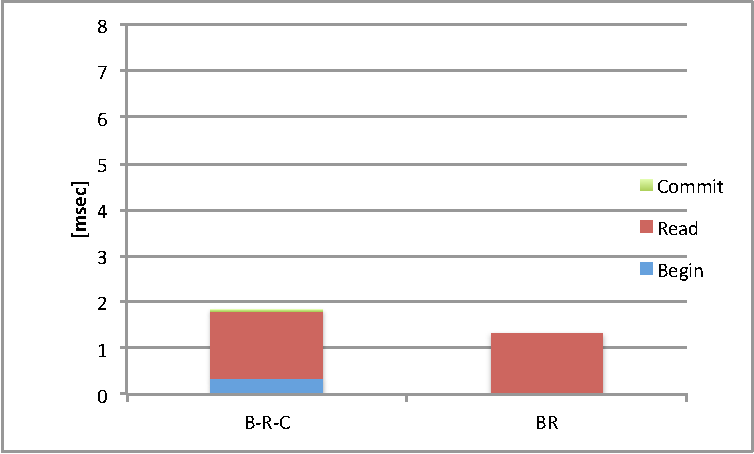
\includegraphics[width=\textwidth]{figs/read_latency.pdf}
%% 	\caption[]{Read}
%%     \label{fig:latency:read}
%%   \end{subfigure}
%%   \begin{subfigure}[t]{0.3\textwidth}
%% 	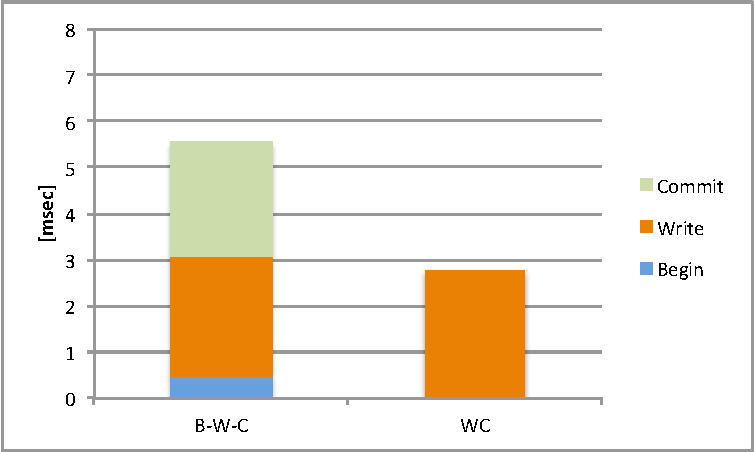
\includegraphics[width=\textwidth]{figs/write_latency.pdf}
%% 	\caption[]{Write}
%%         \label{fig:latency:write}
%%   \end{subfigure}	
%%   \begin{subfigure}[t]{0.3\textwidth}
%% 	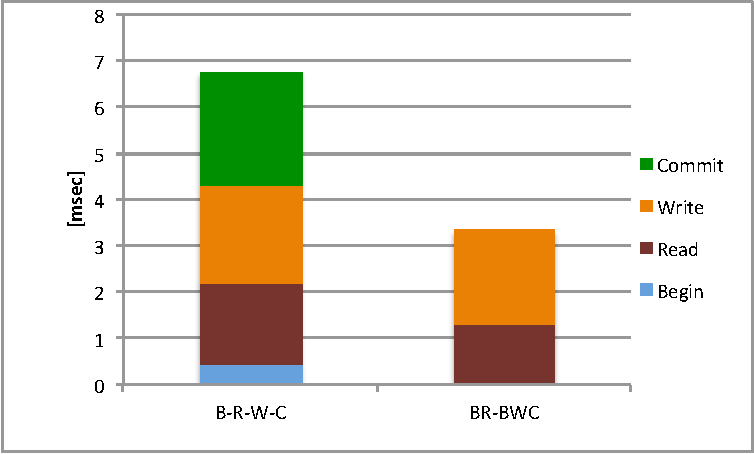
\includegraphics[width=\textwidth]{figs/rmw_latency.pdf}
%% 	\caption[]{Read Modify Write}
%%     \label{fig:latency:rmw}
%%   \end{subfigure}			
%%   \caption{Breakdown of transaction latency}
%%   \label{fig:latency}
%% \end{figure*}

\begin{figure}
\caption{\bf{Experiment architecture.}}
\label{fig:experiment}
\end{figure}

\begin{figure}[!h]
  \centering
  \begin{subfigure}[t]{0.4\textwidth}
	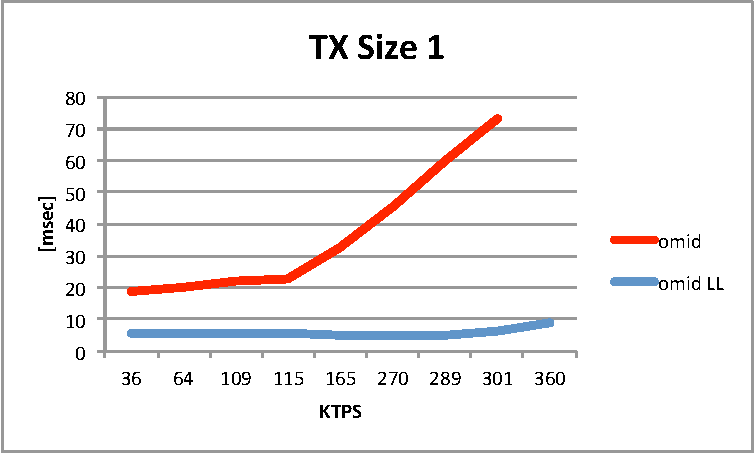
\includegraphics[width=\textwidth]{figs/omdLL1.pdf}
	\caption[]{Transaction of size 1 latency}
    \label{fig:ll:tx1}
  \end{subfigure}
  \begin{subfigure}[t]{0.4\textwidth}
	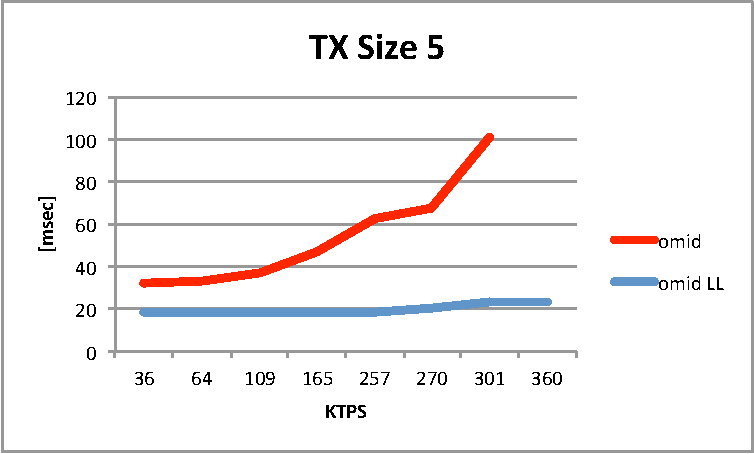
\includegraphics[width=\textwidth]{figs/omdLL5.pdf}
	\caption[]{Transaction of size 5 latency}
    \label{fig:l:tx5}
  \end{subfigure}
    \begin{subfigure}[t]{0.4\textwidth}
	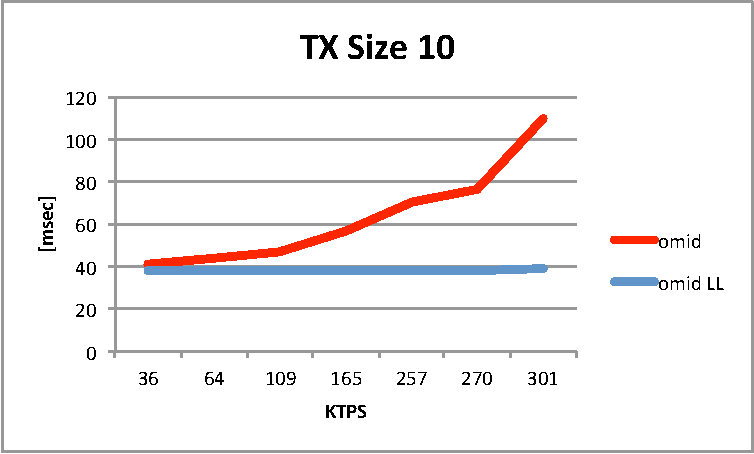
\includegraphics[width=\textwidth]{figs/omdLL10.pdf}
	\caption[]{Transaction of size 10 latency}
    \label{fig:l:tx10}
  \end{subfigure}			
  \caption{A Comparison between Omid's centralized transaction entry and \sys's distributed transaction entry.}
  \label{fig:throughput-latency}
\end{figure}



\begin{figure*}[]
  \centering
  \begin{tabular}{cccc}
    
  \begin{subfigure}[t]{0.4\textwidth}
	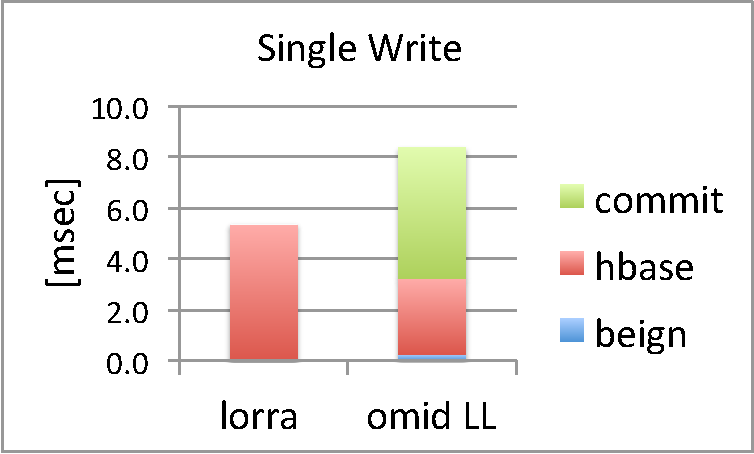
\includegraphics[width=\textwidth]{figs/singlewrite.pdf}
	\caption[]{Single write transactions}
    \label{fig:latency:lorra1write}
  \end{subfigure} &

  \begin{subfigure}[t]{0.4\textwidth}
	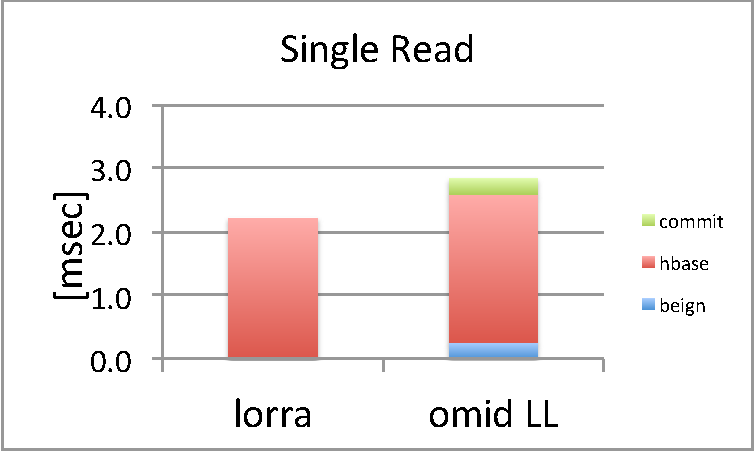
\includegraphics[width=\textwidth]{figs/singleread.pdf}
	\caption[]{Single read transactions}
    \label{fig:latency:lorra1read}
  \end{subfigure} \\

    \begin{subfigure}[t]{0.4\textwidth}
	\includegraphics[width=\textwidth]{figs/lorravslltx5.pdf}
    \caption[]{Transaction size 5}
    \label{fig:latency:read}
    \label{fig:latency:lorra5}
  \end{subfigure} &

  \begin{subfigure}[t]{0.4\textwidth}
	\includegraphics[width=\textwidth]{figs/lorravslltx10.pdf}
    \caption[]{Transaction size 10}
    \label{fig:latency:lorra10}
  \end{subfigure} \\
  
    
  \end{tabular}
  \caption{Latency of \sys\ and \sysll\ }
\end{figure*}

We now evaluate {\sys}'s performance for both the generic and the fast-path transactions, 
focusing on average transaction latency under a variety of workloads. We compare {\sys\/} 
to the mainstream Omid implementation. Both systems use HBase as KV-storage backend.

We run the experiments on 12-core Intel Xeon 5 machines with 46GB RAM and 4TB 
SSD storage. Every node runs the HBase and the underlying Hadoop filesystem (HDFS) 
serving tiers within 8GB JVM containers. 

% Philosophy
\paragraph{Methodology}
We project the transaction performance in a very large production KV-store in which the data (read/write) 
requests are roughly load-balanced. To this end, horizontal scaling of the KV-store and its workload do not 
affect the performance of the data requests. The control (begin/commit) requests are served by the centralized 
TM; scaling the workload congests this bottleneck. We can therefore capture the end-to-end transaction latency
in the projected system with a small HBase cluster that serves a fraction of workload, while stressing the TM 
by a full load of control requests. 

We emulate a 1000-node HBase with a 3-server cluster that processes $0.3\%$ of the projected workload. 
This traffic is driven by the popular YCSB benchmark~\cite{Cooper:2010:BCS:1807128.1807152} 
that exercises the traditional (synchronous) transaction processing API. YCSB measures the end-to-end latencies.
The remainder of the control requests (background load on the TM) are generated by a custom tool~\cite{Omid2017} 
that asynchronously posts them on the wire, and collects the TM responses. Both workload
drivers exploits up to 3 client nodes. Figure~\ref{fig:experiment} depicts the experiment's architecture. 

Our test cluster stores approximately 23M keys, which amounts to 7.66B keys in the emulated system. 
The values are 2K big, which translates to roughly 46GB data, replicated three-way in HDFS. The keys are hash-partitioned
across the servers, thereby balancing the amount of data governed by each server. The data accesses are 50\% reads and 
50\% writes. The key access frequencies follow a Zipf distribution, generated following the description in~\cite{Gray:1994:QGB:191839.191886}. 
The Zipf parameter is $\theta=0.8$ (derived from production workloads). The resulting distribution is very heavy-tailed, which 
guarantees that neither of the servers suffers an excessive portion of traffic due to super-popular items, i.e., the 
data requests are load-balanced, similarly to the data itself.  

Transaction size (number of reads and writes) is a Zipfian distribution with $\theta=0.99$ and a cutoff at 10. 
In this context, e.g., 63\% of the transactions access 3 keys or less, whereas 3\% access 10 keys. 

\paragraph{Generic Transactions} We first focus on the latency of conventional transactions. 
Figure~\ref{fig:throughput-latency}(a-c) depicts the average latency of transactions that perform 1, 5, and 10 
data accesses, respectively. The system loads vary from 35 to 350 transactions per second. We see that 
{\sys\/} scales almost infinitely whereas Omid suffers from a well-pronounced TM bottleneck.   

throughput-la

\remove{
\paragraph{Distributed transaction entry}
We first compare \sys's distributed transaction entry approach to Omid's centralized approach. Figure~\ref{fig:ll} shows the latency of a transaction while applying increasing load on the system. The load is measured in kilo transactions per second (KTPS), and the transaction latency is measured in milliseconds. Figure~\ref{fig:ll:tx1} shows the latency of a transaction with a single read or write. The figure shows that latency obtained by \sys\ is \speedup{4} faster than Omid 2. \sys\ performs better because Omid 2 is throughput oriented and batches the writes to transaction entries, so on every begin stage the client has to wait for all commits in the batch to get persistent.
Figure~\ref{fig:ll:tx1} shows the latency of transactions with 5 read or write operations. This time the latency obtained by \sys\ is \speedup{1.8} faster than Omid 2. For transactions with 5 operations to an Hbase table, the begin and commit time become negligible.

\paragraph{FP API latency}
Figure~\ref{fig:latency} compares the latency observed by YCSB when running regular and FP transactions.
We focus on 3 types of transactions: (1) Read, (2) Write and (3) Read modify write.

Figures~\ref{fig:latency:read} and \ref{fig:latency:write} show the latency of a single read and write transaction. Regular transactions (b-r-c, b-w-c) query the TSO at the begin and commit stage which add 0.3ms for read transactions and 3ms for write transactions.
Figure~\ref{fig:latency:rmw} compares the latency of a read modify write transaction, once using the FP API (br-bwc) and once using the regular transaction API (b-r-w-c).The begin and commit stage of the regular transaction add 3ms to each transaction.
}






\Yoni{
  --background noise
  --switch order of charts
  --explain that the LL is better for all TPS so it doesn't matter the point we choose to check}
